\documentclass[11pt,aspectratio=169]{beamer}

% Assets
\usepackage[czech]{babel}				% Jazyk
%\usepackage[a-2u]{pdfx}				% Kopírování z pdfka
\usepackage{tikz}						% Schémata automatů
\usetikzlibrary{arrows}
\usepackage{pgfplots}
\pgfplotsset{compat=1.15}
\usepackage{mathrsfs}
\usepackage[utf8]{inputenc}
% \usepackage{textcomp}
\usepackage{hyperref}

%%% FONTS
% \usefonttheme{serif}
% \usepackage{lmodern}
\usepackage{helvet}
\usefonttheme[onlymath]{serif}

\hypersetup{%
    pdfencoding=auto,
    pdfauthor={\insertauthor},
    pdftitle={\insertsubtitle}
}
\usepackage{csquotes}					% české uvozovky
\usepackage{enumerate}					% enumerate environment
\usepackage{indentfirst}
\usepackage{mathtools}
\usepackage{pifont}
\usepackage{soul}
\usepackage{xcolor}
\usepackage{graphicx}
\usepackage{amsmath}
\usepackage{subfig}
\usepackage{multicol}

\usepackage{listings}                   % Úryvky z kódu
% Enumerate
%\setlist[enumerate]{topsep=0pt,itemsep=-1ex,partopsep=1ex,parsep=1ex,label=(\arabic*)}
\setbeamertemplate{enumerate items}[circle]

% \MakeOuterQuote{"}

% Colors
\definecolor{lightblue}{HTML}{009AD4}
\definecolor{darkgreen}{HTML}{0D7103}
\definecolor{lightgreen}{HTML}{68FF00}
\definecolor{darkgreen}{HTML}{00D500}
\definecolor{darkred}{HTML}{AF0B0B}
\definecolor{lightred}{HTML}{FF5100}
\definecolor{orange}{HTML}{FFE000}
\definecolor{codeblue}{HTML}{FF0055}
\definecolor{codegreen}{rgb}{0,0.6,0}
\definecolor{codegray}{rgb}{0.5,0.5,0.5}
\definecolor{codebeige}{HTML}{D4A000}
\definecolor{codepink}{HTML}{FF0055}
\definecolor{backcolour}{rgb}{0.95,0.95,0.92}

\newcommand{\markred}[1]{\textcolor{lightred}{#1}}
\newcommand{\markgreen}[1]{\textcolor{darkgreen}{#1}}
\newcommand{\markorange}[1]{\textcolor{orange}{#1}}
\newcommand{\markblue}[1]{\textcolor{lightblue}{#1}}

% Inline images
\newcommand{\inlineimgscale}{1.1}

% X and check mark
\newcommand{\cmark}{\markgreen{\ding{51}}}
\newcommand{\xmark}{\markred{\ding{55}}}

% Math
\newcommand{\R}{\mathbb{R}}
\newcommand{\C}{\mathbb{C}}
\newcommand{\N}{\mathbb{N}}
\newcommand{\Z}{\mathbb{Z}}
\newcommand{\Q}{\mathbb{Q}}

\newcommand{\compl}[1]{#1^\complement}
\newcommand{\mapping}[3]{#1:#2 \rightarrow #3}
\newcommand{\mapto}[3]{#1:#2 \mapsto #3}
\newcommand{\set}[1]{\left\{#1\right\}}

% TODO
\newcommand{\todo}[1]{\textcolor{red}{(\noindent TODO: #1.)}}

% Code
\lstdefinestyle{python}{
    language=Python,
    basicstyle=\small\ttfamily\color{black}, % Standardschrift
    tabsize=2, % Groesse von Tabs
    extendedchars=true, %
    breaklines=true, % Zeilen werden Umgebrochen
    %keywordstyle=\color{red}\bfseries,
    %keywordstyle=[1]\textbf, % Stil der Keywords
    % keywordstyle=[2]\textbf, %
    % keywordstyle=[3]\textbf, %
    % keywordstyle=[4]\textbf, \sqrt{\sqrt{}} %
    stringstyle=\color{codebeige}\ttfamily, % Farbe der String
    showspaces=false, % Leerzeichen anzeigen ?
    showtabs=true, % Tabs anzeigen ?
    xleftmargin=17pt,
    framexleftmargin=17pt,
    framexrightmargin=5pt,
    framexbottommargin=4pt,
    commentstyle=\color{darkgreen},
    % morecomment=[s][\color{green}]{#}{},
    %backgroundcolor=\color{grey},
    showstringspaces=false, % Leerzeichen in Strings anzeigen ?
    %morekeywords={__global__} % CUDA specific keywords
    morekeywords={False, None, True, and, as, assert, async, await, break, class, continue, def, del, elif, else, except, finally, for, from, global, if, import, in, is, lambda, nonlocal, not, or, pass, raise, return, try, while, with, yield}, % list your attributes here
    keywordstyle=\color{codepink},
    identifierstyle=\color{blue}
}
\lstdefinestyle{sharpc}{
    language={csh},
    basicstyle=\small\ttfamily\color{black}, % Standardschrift
    tabsize=2, % Groesse von Tabs
    extendedchars=true, %
    breaklines=true, % Zeilen werden Umgebrochen
    %keywordstyle=\color{red}\bfseries,
    %keywordstyle=[1]\textbf, % Stil der Keywords
    % keywordstyle=[2]\textbf, %
    % keywordstyle=[3]\textbf, %
    % keywordstyle=[4]\textbf, \sqrt{\sqrt{}} %
    stringstyle=\color{blue}\ttfamily, % Farbe der String
    showspaces=false, % Leerzeichen anzeigen ?
    showtabs=true, % Tabs anzeigen ?
    xleftmargin=17pt,
    framexleftmargin=17pt,
    framexrightmargin=5pt,
    framexbottommargin=4pt,
    commentstyle=\color{blue},
    % morecomment=[s][\color{green}]{//}{},
    %backgroundcolor=\color{grey},
    showstringspaces=false, % Leerzeichen in Strings anzeigen ?
    %morekeywords={__global__} % CUDA specific keywords
    morekeywords={abstract, event, new, struct, as, explicit, null, switch, base, extern, object, this, bool, false, operator, throw, break, finally, out, true, byte, fixed, override, try, case, float, params, typeof, catch, for, private, uint, char, foreach, protected, ulong, checked, goto, public, unchecked, class, if, readonly, unsafe, const, implicit, ref, ushort, continue, in, return, using, decimal, int, sbyte, virtual, default, interface, sealed, volatile, delegate, internal, short, void, do, is, sizeof, while, double, lock, stackalloc, else, long, static, enum, namespace, string}, % list your attributes here
    keywordstyle=\color{cyan},
    identifierstyle=\color{red}
}
\lstdefinestyle{clang}{
    basicstyle=\small\ttfamily\color{white},
    language=C,
    keywordstyle=\color{codeblue},
    commentstyle=\color{codegreen},
    numberstyle=\tiny\color{codegray},
    stringstyle=\color{codebeige},
    breakatwhitespace=false,
    breaklines=true,
    captionpos=b,
    keepspaces=true,
    numbersep=5pt,
    showspaces=false,
    showstringspaces=false,
    showtabs=false,
    morekeywords={void,int,double,float,unsigned,if,else,\#include}
    tabsize=0.5
}
\lstset{escapeinside={(*}{*)},style=clang}

\newcommand{\hlcode}[1]{\colorbox{red}{#1}}
% Beamer theme
\usetheme{Darmstadt}
\useoutertheme[subsection=false]{miniframes}
\definecolor{themecolor}{HTML}{3B6C3B}
\usecolortheme[named=themecolor]{structure}
\setbeamertemplate{frame numbering}[fraction]
\setbeamertemplate{navigation symbols}{}

% Blocks
\setbeamertemplate{blocks}[default]
\setbeamercolor{block title}{bg=blue, fg=white}
% \setbeamertemplate{blocks}[rounded][shadow=false]

% Title page
\title{\textsc{Analytická geometrie a SVG}}
\author{Adam Papula, David Weber}
\institute{SPŠE Ječná, MFF UK}
\date{\today}

\begin{document}

    % Title page
    {
        \setbeamertemplate{footline}{}
        \maketitle
    }
    \addtocounter{framenumber}{-1}

    % Table of contents
    \begin{frame}[t]{Obsah}
        \tableofcontents
    \end{frame}

    \section{Pravidla dobrého návrhu}
    \subsection{Fáze efektivní tvorby dokumentu}
    \begin{frame}[t]{Pravidla dobrého návrhu}
        \onslide<2->{Fáze efektivní tvorby dokumentu většího rozsahu:}
        \onslide<3->{
            \begin{itemize}
                \onslide<3->{\item \emph{Značkování} (struktura dokumentu)}
                \onslide<4->{\item \emph{Návrh} (formát papíru, okraje, písma, řádkování, \dots)}
                \onslide<5->{
                    \begin{itemize}
                        \item V podstatě přiřazujeme vizuální význam (sémantiku) značkám
                    \end{itemize}
                }
                \onslide<6->{\item \emph{Sazba} (``nalití'' obsahu do vyhrazených chlívků v dokumentu za dodržení typografických pravidel)}
                \onslide<7->{\item \emph{Korektura} (popř. se vracíme zpět k sazbě)}
                \onslide<8->{\item \emph{Tisk/publikace}}
            \end{itemize}
        }
    \end{frame}
    
    \subsection{Ukázka značkování}
    \begin{frame}[fragile]{Značkování}{v jazyce \textbf{Markdown}}
        \begin{verbatim}
# Nadpis 1

## Nadpis 2

### Nadpis 3

Tohle je *kurzíva*.

Toto je **tučný** text.

- Seznam
- Položka 1
- Položka 2
        \end{verbatim}
    \end{frame}

    \section{Sazba počítačem}
    \begin{frame}[t]{Sazba počítačem}
        \only<2-6>{
            \only<2-6>{
                \begin{itemize}
                    \only<2->{\item Dnes tvoří dokumenty skoro každý}
                    \only<3->{\item $\implies$ Software sazbu značně zjednodušil}
                    \only<4->{\item Prakticky odpadla nutnost značkovat}
                    \only<5->{\item WISIWYG $\times$ WISIWYM}
                    \only<6->{
                        \begin{itemize}
                            \item \emph{What You See Is What You \textbf{Get}}
                            \item \emph{What You See Is What You \textbf{Mean}}
                        \end{itemize}
                    }
                \end{itemize}
            }
        }
        \only<7>{
            \begin{figure}
                \centering
                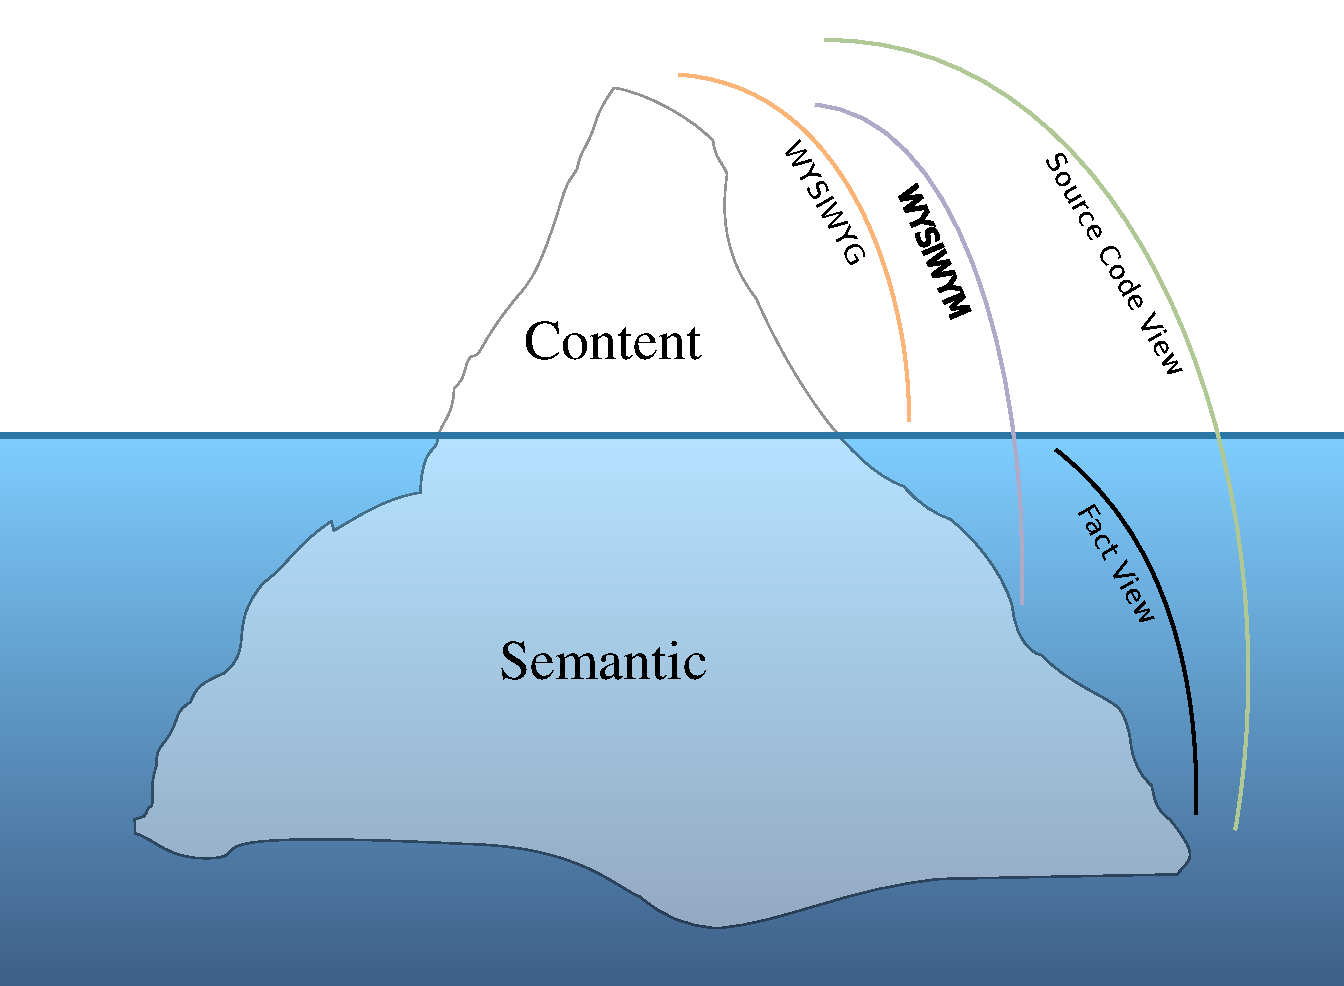
\includegraphics[scale=.4]{image/ViewsIceberg.pdf}
            \end{figure}
        }
    \end{frame}

    \section{Historie \TeX u v kostce}
    \begin{frame}[t]{Trošku do historie\dots}
        \only<2->{
            \begin{itemize}
                \only<2->{\item Systém \TeX{} vznikl v 70. letech, kdy \emph{Donald E. Knuth} (USA) byl zklamán z kvality tehdejší sazby jeho skript (chyby ve vzorcích, typografie).}
                \only<3->{\item V roce 1977 přichází s vlastním sázecím systémem (sepisuje základní funkce)}
                \only<4->{\item O rok později (1978) vychází první verze systému \TeX{}.}
            \end{itemize}
        }
    \end{frame}
    \begin{frame}[t]{Trochu k vývoji \TeX u\dots}
        \only<2->{
            \begin{itemize}
                \only<2->{\item 1978 -- první verze systém \TeX}
                \only<3->{
                    \begin{itemize}
                        \item Obsahoval cca 300 základních příkazů (dosti složité programování $\impliedby$ low-level)
                        \item Příkazy typu \emph{``skoč doprava/doleva o x pozic'', vypiš posloupnost znaků, změň písmo, \dots}
                        \item Pro běžného uživatele téměř nepoužitelný
                    \end{itemize}
                }
                \only<4->{\item 1987 -- \TeX{} v dnešní podobě (od té doby nezměněn)}
                \only<5->{\item Z důvodu uživatelské nepřivětivosti vzniká plain\TeX
                \begin{itemize}
                    \item Obsahuje cca 900 příkazů
                \end{itemize}}
                \only<6->{\item Nejvíce se však podařilo protlačit systém šírší veřejnosti \emph{Laslie Lamportovi}, který uvedl tzv. \LaTeX{} (rok 1985)}
                \only<7->{
                    \begin{itemize}
                        \item Balíček maker ke standardnímu \TeX u.
                        \item Uživatel se více mohl soustředit na obsah $\implies$ formu zajišťují předchystaná makra.
                    \end{itemize}
                }
            \end{itemize}
        }
    \end{frame}

    \section{Specifika \TeX u}

    \subsection{Co je \TeX}
    \begin{frame}[t]{Co je \TeX}
        \begin{itemize}
            \item Sázecí systém
            \item Programovatelný (každé makro si lze přizpůsobit)
            \item Dávkový: \emph{textový soubor $\rightarrow$ grafický výstup}
            \item Portabilní (nezávislý na verzi souboru)
        \end{itemize}
    \end{frame}

    \subsection{Co není \TeX}
    \begin{frame}[t]{Co naopak \TeX{} není}
        \only<2->{
            \begin{itemize}
                \only<2->{\item Editor}
                \only<3->{\item Program na úpravu grafiky}
                \only<4->{
                    \begin{itemize}
                        \item Existuje program \emph{Ipe}, který je plně kompatibilní se sazbou v \TeX uvedl
                    \end{itemize}
                }
                \only<5->{\item WISIWYG}
                \only<6->{\item rychle naučitelný}
            \end{itemize}
        }
        \only<6->{
            \begin{figure}
                \centering
                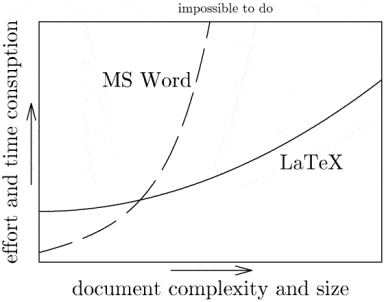
\includegraphics[scale=.4]{image/fig_word-vs-latex.png}
            \end{figure}
        }
    \end{frame}

    \subsection{Ukázka}
    \begin{frame}[fragile]{Ukázka \TeX ového kódu}
        \begin{verbatim}
\documentclass{article}
\begin{document}

\title{Dokument v LaTeXu}
\author{David Weber}
\date{\today}
\maketitle

\section{Úvod}
Lorem ipsum dolor sit amet, consectetur adipiscing elit...

\subsection{První podsekce}
Lorem ipsum dolor sit amet, consectetur adipiscing elit...

\end{document}            
        \end{verbatim}
    \end{frame}

    \begin{frame}{Výsledek\dots}
        \begin{figure}
            \centering
            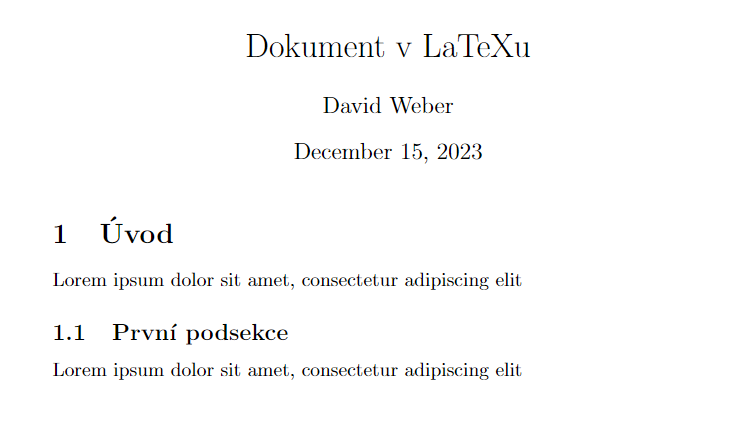
\includegraphics[scale=.5]{image/ukazka_latex.png}
        \end{figure}
    \end{frame}

    \section{Porovnání \LaTeX u a Wordu}
    \begin{frame}{Pokud o porovnání \LaTeX u a Wordu}
        \only<2->{
            \begin{itemize}
                \only<2->{\item Není WISIWYG}
                \only<3->{\item Z počátku trvá déle se \LaTeX{} naučit}
                \only<4->{\item Složitější instalace}
                \only<5->{
                    \begin{itemize}
                        \item Existují však různé online nástroje pro práci s \LaTeX em, např. \emph{Overleaf}
                    \end{itemize}
                }
                \only<6->{\item Kvalitnější sazba matematických a jiných symbolů}   
                \only<7->{\item Nezávislý na verzi}
                \only<8->{\item \LaTeX{} nutí částečně uživatele značkovat (oddělit obsah od formátu)}
                \only<9->{\item Plovoucí obrázky a tabulky}
            \end{itemize}
        }
        \only<10->{
            \begin{itemize}
                \item Pro opakované prvky lze zavést vlastní makro
                \item Velké množství dostupných extérních balíčků
                \item Cena
            \end{itemize}
        }
    \end{frame}

    \section{K čemu se \LaTeX{} hodí}
    \begin{frame}[t]{K čemu se \LaTeX{} hodí\dots}
        \only<2->{
            \begin{itemize}
                \only<3->{\item Matematická/technická sazba}
                \only<4->{\item Výzkumné práce, protokoly}
                \only<5->{\item Závěrečné práce}
                \only<6->{\item Skripta}
                \only<7->{\item Prezentace}
                \only<8->{\item (Automatizované) generování dokumentů}
                \only<9->{\begin{itemize}
                    \item Např. testy pro studenty (každá varianta jiné otázky/příklady).
                \end{itemize}}
            \end{itemize}
        }
    \end{frame}

\end{document}